
% Change the style for the front page, put in a background image.
\setbeamertemplate{background canvas}{%
  %\includegraphics[width=\paperwidth]{title-tip_2-dark}}
%  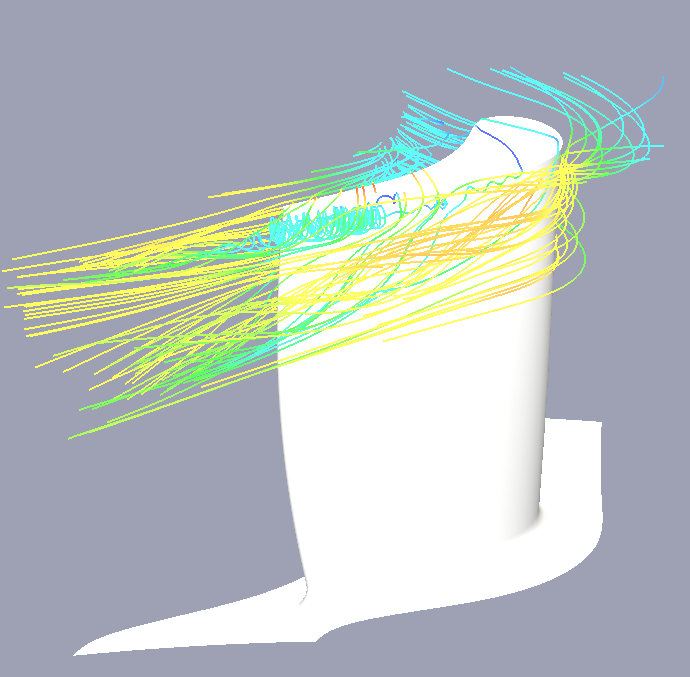
\includegraphics[width=\paperwidth]{title-tip_2-bright}}
    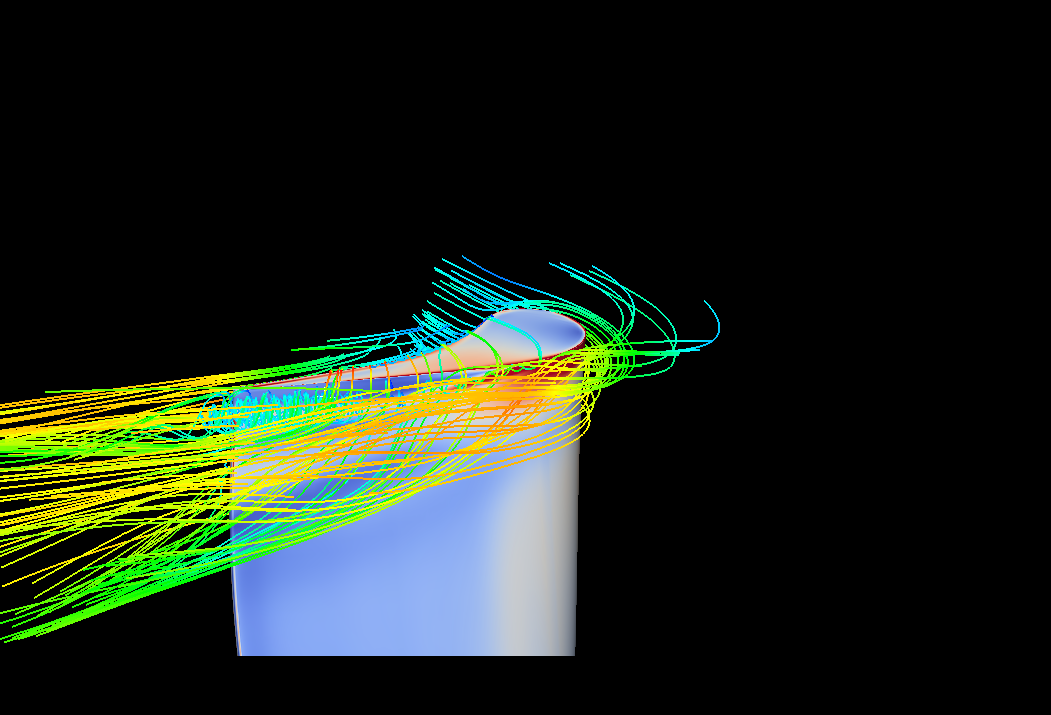
\includegraphics[width=14.2cm]{streamline7.png}}

\begin{frame}[plain]
  % titlepage; move things around to suit the image.
  % in this template a white font is used, thence the image
  % was darkened (gimp is your friend), and a white on dark logo
  % variant is used.
\vfill\vfill
\leftline{\color{white}\huge\bf Stabilisation of a discrete adjoint}
\center{\color{white}\huge\bf using implicit timestepping}
\vfill\vfill
\vfill\vfill\vfill\vfill

\rightline{\color{white}\bf Shenren Xu}
\rightline{\color{white}\bf Jens-Dominik M\"{u}ller}
\rightline{\color{white}\bf {Queen Mary, University of London}}
\vfill\vfill

\begin{columns}
  \begin{column}{.3\textwidth}
%    \includegraphics[width=\linewidth]{QM144BlueOnLight}
%   
\includegraphics[width=\linewidth]{ccfd3}
%	
\includegraphics[width=\linewidth]{WUT_L}
  \end{column}
  \begin{column}{.6\textwidth}
    \rightline{\color{white}\large \bf hydra implict meeting}
    \rightline{\color{white}\large \bf Derby, 10 April 2014}    
  \end{column}

\end{columns}


\end{frame}
\setbeamertemplate{background canvas}[default]
